\documentclass[runningheads]{llncs}

\usepackage[utf8]{inputenc}
\usepackage[ngerman, english]{babel}

\usepackage[T1]{fontenc}
\usepackage{amssymb}
\setcounter{tocdepth}{3}
\usepackage{graphicx}
\usepackage{amsmath}
\usepackage{mathcomp}
\usepackage{url}
\usepackage[chapter]{algorithm}
\usepackage{algorithmic}
\usepackage{subfigure}

\usepackage{appendix}

\usepackage{listings}
\lstset{numbers=left, numberstyle=\tiny, numbersep=5pt}

\newboolean{showcomments}
\setboolean{showcomments}{true} % SET TO false for camera-ready
\ifthenelse{\boolean{showcomments}}
  { \newcommand{\nbnote}[2]{
      \fbox{\bfseries\sffamily\scriptsize#1}
      {\sf\small$\blacktriangleright$\textit{#2}$\blacktriangleleft$}
    }
  }
  { \newcommand{\nbnote}[2]{}
  }
\newcommand\todo[1]{\nbnote{TO DO}{#1}}

\begin{document}
\mainmatter
\title{Trends and Concepts in the Software Industry II: \\ Development of Enterprise Software}
\author{Team 5: Providing Data Context During Development}
\institute{Thomas B\"unger, Felix Leupold, Johan Uhle, \\ Patrick Schilf, Lauritz Thamsen, Fabian Tschirschnitz \\[0.1in] Johannes Wust \\
Franziska Haeger, Dr. Anja Bog, Dr. Juergen M\"uller, Prof. Hasso Plattner \\
Hasso-Plattner Institute \\[0.1in]
March 15, 2013}
\date{March 15th, 2013}
\maketitle

\newpage

\tableofcontents
\newpage

%Head of Documentation - Patrick: gerade ziehen

\section{Introduction}
%HoD
%Seminar, Seminarablauf, Thema (= deren how might we question)
%(dabei Bezug zu unserem Subthema aufbauen)
% close with an outline of this document, include references to all sections, see lables

%!TEX root = ../document.tex

\section[Design Thinking (Author: Felix Leupold)]{Design Thinking}
\label{sec:DESIGN_THINKING}

\emph{Design thinking} refers to the method of finding an innovative solution to an abstract or ill-defined problem. It attempts to structure the ideation process and provides guidelines, methodologies and frameworks that help in problem forming, -solving and -design. Design thinking is a human-centered approach with multidisciplinary collaboration and iterative improvements to produce innovative products, systems and services \cite{design_thinking_book}. There are various interpretations and definitions of design thinking. We refer to design thinking as defined by the Hasso Plattner Institue of Design at Stanford and Potsdam. In this definition the design thinking process contains six different phases, which are pictured in Figure \ref{fig:design_thinking_process}. The process is not linear, which is indicated by the connections amongst different non-succeeding phases. Every instance of a design thinking project is different. It is possible to jump back and forth between the different phases as you encounter new inflection points. 

%nochmal �berdenken
In the following, we briefly explain the aim of each phase as they also reflect the pathway in the course of our project and the structure of this report.

\begin{figure}
    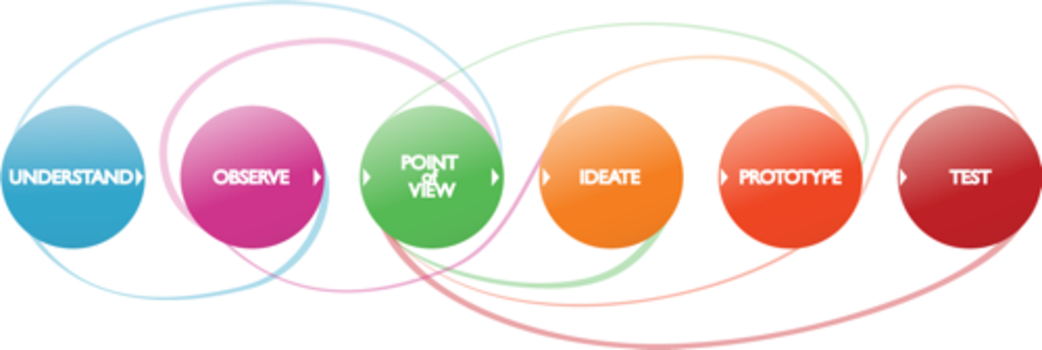
\includegraphics[width=\linewidth]{images/design_thinking_process}
    \caption{Design Thinking process according to \emph{Hasso Plattner Institue of Design} at Stanford and Potsdam.}
    % #selfrespect
    \label{fig:design_thinking_process}
\end{figure}

\paragraph{Understand}
In the first phase of the process, the team becomes familiar with the problem domain by talking to experts and conducting research. The goal is to develop background knowledge through these experiences. It is the foundation for all further steps. Throughout the process this stage might be visited again as new areas of problems, ideas or solutions emerge.

\paragraph{Observe}
What people say does not always correspond to their actual feelings, thoughts or actions. Therefore, it is necessary to watch how people behave and interact. These observations can be used to talk to users, ask questions and reflect on their behaviors. They lay the foundation for insights which are needed to define a point of view later in the process. Another point of this phase is to develop a kind of empathy for the user.

\paragraph{Point Of View}
The point of view consists of three parts: A persona, which is a concrete specification of the target user the team is designing for. Second, a need that this persona has and that the team is trying to satisfy with its solution. Lastly, an insight that has been generated from the observation made in the second phase. A commonly used method of defining a point of view is the "How might we..." question, which is a statement in a form "How might we help our persona to satisfy his or her need".
While the preceding phases tried to capture a wide range of users and problems, in this stage the team settles on a single point from which it can converge again in the next phase.

\paragraph{Ideate}
While the first three phases focus on defining and understanding the problem, the ideation phase opens up the solution space for the problem. The team is challenged to brainstorm as many solutions as possible by going for quantity, deferring judgment and building on the ideas of others.

\paragraph{Prototype}
Prototyping is a crucial part of the design thinking process. It allows to make the ideas visible and tangible. Quick and cheap prototypes, e.g. sketches on paper, are well suited for conveying the idea and getting feedback. People tend to hesitate to criticize or suggest changes for overly polished prototypes. A key concept is to fail early and often.

\paragraph{Test}
In the test phase the team collects feedback on their ideas which they made experienceable through their prototype. The goal of this phase is to learn which parts of the design work and which don't.
Testing ensures that the product is desirable for the end user and stresses the user focus of design thinking.
Latest from here on the team continues with one of the earlier phases.

\paragraph{}
Each potential solution has to satisfy three requirements as depicted in Figure \ref{fig:desire_viable_feasible}. Desirability ensures, it addresses an actual need of the user. Feasibility means that the solution should be technically possible to implement. Lastly, it has to be viable for the business partner providing the solution.
Innovative solutions lie in the intersection of the three sets. Design thinking helps to find solutions that lie in this intersection.

\begin{figure}[H]
\begin{centering}
    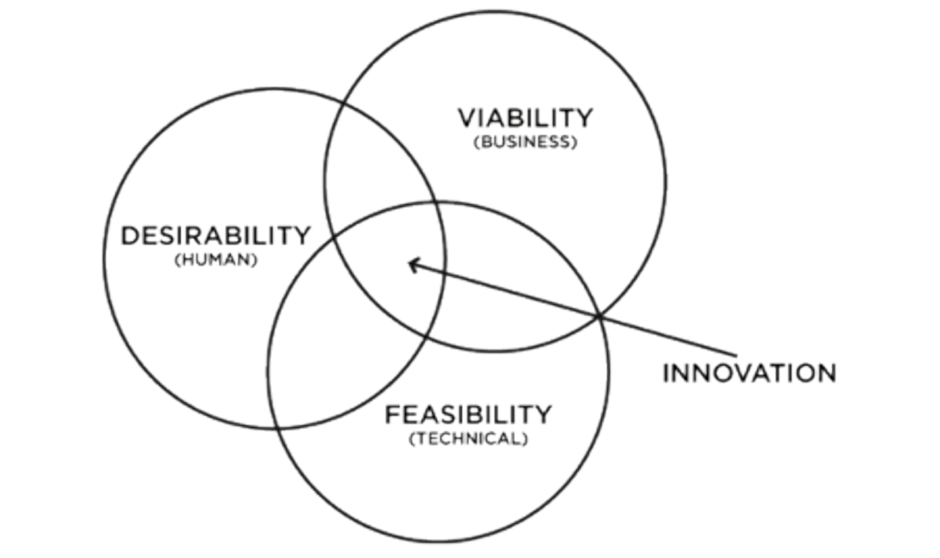
\includegraphics[width=0.5\linewidth]{images/desire_viable_feasible}
    \caption{Solution can be categorized into different sets. An innovative solution has to be viable, desirable and feasible.}
    % #selfrespect
    \label{fig:desire_viable_feasible}
\end{centering}
\end{figure}
%intro to Design Thinking, its cycle and some intro to our results


\section{Understand} \label{sec:UNDERSTAND}
%Johan
%!TEX root = ../document.tex
In the first phase of our research, we interviewed various people in sofware companies. In this section we will summarize the interviews and the insights we gained from them.

% TODO: Programmers name?
\paragraph{XXXXX from Psipenta}
Psipenta builds an ERP system for SMBs with a focus on manufactoring and suppy chain management. Their core product was developed initially in Cobol and parts have later been and still being ported to C++ and Java. Development happens largely in Eclipse, which has been largly extended and customized by Psipenta with automated code generation and integration into their workflow and environment. Work is flexible with home and remote work.

Our interview partner was XXXX. He is working on porting parts of the old code from Cobol to Java as well as developing entirely new features.

XXXXX estimates the time spent in daily communication at around 30\%. This includes answering emails and attending meetings with coleagues.

In the interview XXXX put an emphasis on code quality. A core means to achieve this was automated testing, best even with involving the customer.

As major churns, XXX mentioned interruptions, from co-workers as well as from a slow and/or unintuitive tool chain. As example he mentioned that building a running version of his product to manually test it takes more than half an hour.

\paragraph{Nicole von Steht from SAP}
SAP is one of the biggest enterprise application companies in the world. Nicole works as Frontend application developer at SAP. Her team consists of 12 people and uses the Scrum methodology. The team is located on one floor and most communication happens face-to-face.

Code quality is a core value, that is assured by unit and integration testing with continuous integration as well as rotating pair programming. Nicole writes code in a customized version of Eclipse.

\paragraph{Tillman Giese from SAP}
Tillman is working at SAP on the HANA Security Engine. His team consists of 8 people and is split over 2 offices.

Tillman regularly deals with other teams globally distributed, which is often difficult because of time zone differences. He is getting a lot of support requests, which he said most of the time are answered questions that the rquester could have been able to resolve themselves, if they would have just put in effort to research the question correctly. Often, the requests interrupt his workflow. To illustrate this state, Tillman said: \emph{I wish I could work on one task for a full hour}.

As a side project, Tillman is running Agile development workshops at SAP.

\paragraph{Frank Brunswig from SAP}
Frank is working as Chief Architect at SAP. He's been involved with the company fro 20 years already, worked on various projects and currently oversees the creation of the AppBuilder platform, which enables the creation of custom mobile applications.

Apart from doing small prototype implementations to evaluate a new technology, Frank does not code regularly. His work mainly happenes on a organizational level, where he performs requirement anaysis, organizes his teams, maintains the cross-organizsation-alignment and finds cross-team synergies.

For coding and in his teams Frank prefers all-in-one IDE solutions, which in the best case integrate the complete workflow from finding the requirements over writing code to the final deployment.

His major problem in development are unclear or changing requirements. He is also not an advocate of Agile Methodology, because they badly distribute responsibilities and make the development process harder to control.

\paragraph{Christof Dorner from Readmill}
The Berlin-based startup Readmill that builds an ebook reader and social network around that. Christof is Backend Developer for the Ruby on Rails application. He works in a development team of 4. The team works with the Kanban methodology.

Christof mentioned an interrupted workflow as an important goal for his day-to-day work. To minimize interruptions through his co-workers, they set up an asynchronous company chat where everyone can participate when they feel like it. Also Christof always works with noise-canceling headphones on. He optimized his tools highly to reduce any wasted waiting time while working. This includes customizing his editor and writing small scripts for churn tasks. Furthermore when choosing the technology for Readmill, the whole team takes into account how easy development with this technology will be and makes developer satisfaction an important component of the decision process.

Tests are a core component of Christof's workflow for developing new features or fixing bugs. He does not do straight test-driven development but rather switches between writing code, testing on the console or web app and writing tests as he likes. He puts an emphasis on the fact that all deployed code has a high test coverage. Code review are done via Pull Requests on Github.

As problems while developing, Christof mentioned refactoring of old code (especially tests), reproducing bugs and interruptions of any kind.

\paragraph{Mobile.de}

XXXXXXXXX KEIN PROTOKOLL
%Pre seminar interviews

\section{Observe} \label{sec:OBSERVE}
%Johan
%Bachelor projects, conventional development (edit, build, compile)

%!TEX root = ../document.tex

\section[Point of View (Author: Felix Leupold)]{Point of View} \label{sec:POINT_OF_VIEW}

A point of view (POV) consists of three parts: a concrete specification of the user we are designing for, his or her needs we are trying to satisfy with our solution and finally an insight we derived from the understanding and observation phase. We present all of these in this section.

We derive a \emph{"How might we..."}-question from our POV and try to answer this question during the ideation phase. This description presents our final Persona and her needs. Throughout the course we repeatedly adapted our Persona slightly as we discovered new needs and reevaluated their importance for our persona.

\subsection{Persona}
\label{subsec:persona}

Our Persona is Amber, she is 31 years old and for roughly six years has she been working as a Software Developer at a big company that use HANA as a database for their applications. Within her team of ten developers, she programs applications that work on big data sets and are performance critical. While her main focus is on the backend side, she does not consider herself a database expert. Though she still knows how to write SQL queries, she is not able to predict the impact of certain changes in a query formulation on its performance just by looking at the statement. She works in her favorite development environment studio, which is Eclipse\footnote{\url{http://www.eclipse.org/}}. As a seperate environment, HANA Studio allows her to look at the content or schema of the database.

Amber enjoys coding a lot. It is the favorite part of her work. She is also very enthusiastic and wants to get features completed as fast as possible. She uses a lot of different tools that help her simplify reoccurring tasks and boost her productivity.

However, throughout her work day Amber usually experiences a lot of interruptions. We refer to these interruptions as \emph{Context Switches} that pull her out of her workflow. These might be small switches, like changing from the editor to the browser to browse for something online but can also be bigger ones, such as having to write an email or even physical interruptions caused by colleagues who ask for her attention.

\begin{figure}
    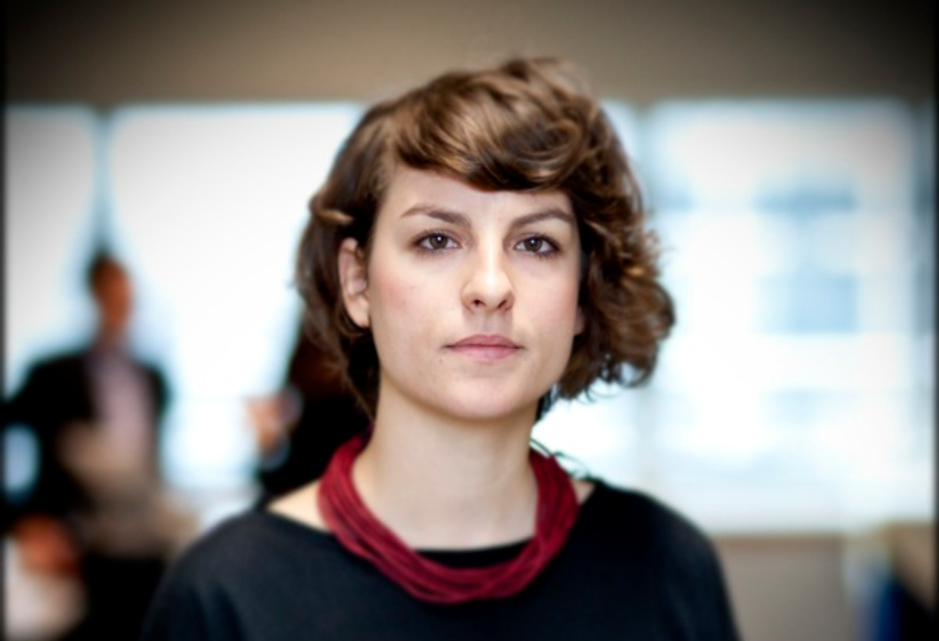
\includegraphics[width=\linewidth]{images/amber}
    \caption{Our Persona Amber, a software developer for performance critical big data applications.}
    % #selfrespect
    \label{fig:amber}
\end{figure}

\subsection{Needs}
Amber's needs are manyfold. The essential ones are:

\begin{itemize}
	\item She wants to do her work in the most efficient way.
	\item Since her applications are performance critical, she needs to evaluate her code against real customer data.
	\item Amber is not an SQL expert. Thus, she needs a way to explore and learn which parts of a query perform well and where bottlenecks are.
	\item She wants her productivity tool chain to be integrated into her IDE in order to avoid switching contexts.
	\item The general number of Context Switches needs to be minimized.
\end{itemize}

Throughout the seminar we down-weighted the importance of the last point as we narrowed down the interruptions that we wanted to tackle. We discovered that although big Context Switches like replying to emails lead to longer disruptions, they occur way less frequently than small Context Switches, such as navigating between applications. Thus tackling issues of the latter type may, accumulated, lead to a big increase in efficiency which is why we focused on that.

\subsection{Insight}

During our observations we saw how our Persona figured out to understand SQL queries written in code. She copied the query from her Eclipse editor into HANA Studio. As in Eclipse her query appears as multiple split \emph{Strings} she has to escape all contained quotes. This is the first Context Switch. Most queries also contain parameters that are bound during runtime. In order to execute the query in HANA Studio Amber looks up appropriate values in the schema. This is the second Context Switch. If the executed query does not behave as expected she is forced to go over this whole process again, switching back and forth in the Studio between edit- and result-view mode. There is no way to recognize the impact of query changes on the result in the same window. Thus, this results in a number of additional Context Switches. If the query finally behaves as desired, Amber has to copy it back into her code editor and turn all concrete values back into variables.

We consider this interaction as a workaround and take it as a foundation for our Point Of View as it emphasizes the most important need. That is predicting the impact of queries on the underlying data. We combine our Persona and her need with one of the insights we gathered during our interviews, namely that \textit{Code needs data context} (cf. Section \ref{sec:OBSERVE}).


\subsection{POV Statement}

\begin{description}
	\item [User] Amber, a productivity junkie, working with HANA on performance critical big data business applications.
	\item [Need] Amber needs to predict the performance and logical impact of her code on the underlying data sets using only without switching to another application.
	\item [Insight] Code needs data context.
\end{description}

Based on this, we derived the following \emph{"How might we question..."}:

\subsection{How Might We...}

\begin{quote}
\emph{"How might we help Amber to predict the impact of her code on real customer data in one integrated development environment?"}
\end{quote}
%Felix

\section{Ideation} \label{sec:IDEATION}
%Felix
%our idea, plus make up some ideas that were not followed

\section{Paper Prototype} \label{sec:PAPER_PROTOTYPE}
%Thomas

\section{User Testing and Feedback} \label{sec:USER_TESTING}
%Thomas
%Testing
%Feedback

\section{Final Prototype} \label{sec:FINAL_PROTOTYPE}
%Fabi

%!TEX root = ../document.tex
\section{Implementation Ideas} \label{sec:IMPLEMENTATION_IDEAS}
%Lauritz
As described in Section~\ref{sec:PAPER_PROTOTYPE} and \ref{sec:FINAL_PROTOTYPE}, our proposed environment always presents relevant runtime data when developers interact with statements.
Just like in a debugger, when developers, for example, hover over identifiers in their application code, the IDE presents actual data, either objects or database rows.
However, in contrast to ordinary debugging environments, developers should not only be able to see the current state and step through the execution, but actually add and evaluate statements.
This should allow an interactive style of development centered around seeing the impact and effects of their code and queries immediately.
These features rely on the availability of runtime data.
First, developers can only see values and database entries for identifiers if such data is available.
Second, statements that might or might not embedd queries require referred variables and potentially even a database to run.
A realization of our idea would, therefore, implement components that gather the necessary data contexts from actual program runs as well as components that support developers in selecting interesting data contexts during development.

\subsection{Gathering Data Contexts}

Our approach depends on the availability of data contexts for the code sections of interest to the developer.
Such data contexts need to be realistic and immediately available to be useful.
Given these premises, two approaches could provide data contexts for specific code sections:
Either, deterministic test runs could establish data contexts on demand or tracing the application's execution could record data contexts in advance.
Running tests to provide the runtime during development would only require to store coverage information that associates code sections with test cases, while recording contextual information in advance implies storing as much data as necessary to actually run any statements in the sources of an application.
The test execution time depends on the granularity of the covering tests with a full spectrum from fine-grained, isolated unit tests to high-level, long-running acceptance tests.
Previously recorded data contexts, however, need just be fetched from a database, which could also be an in-memory database, and, thus, potentially provides faster access to data contexts compared to establishing runtime data through running tests.
Fetching recorded data context is also independent of the availability as well as granularity of tests and could also be captured in deployed systems used by real customers to provide more realistic runtime data.

Assuming deterministic code, a reasonable trade-off between space and time consumption, which we would investigate first, could record data not on the level of single statements but on the level of method scopes.
Such an implementation would record all data necessary to actually run a method with all its statement, including provided parameters, accessible state, and the the database at the moment methods are entered, as shown in Figure~\ref{fig:context_recording}.

\begin{figure}
    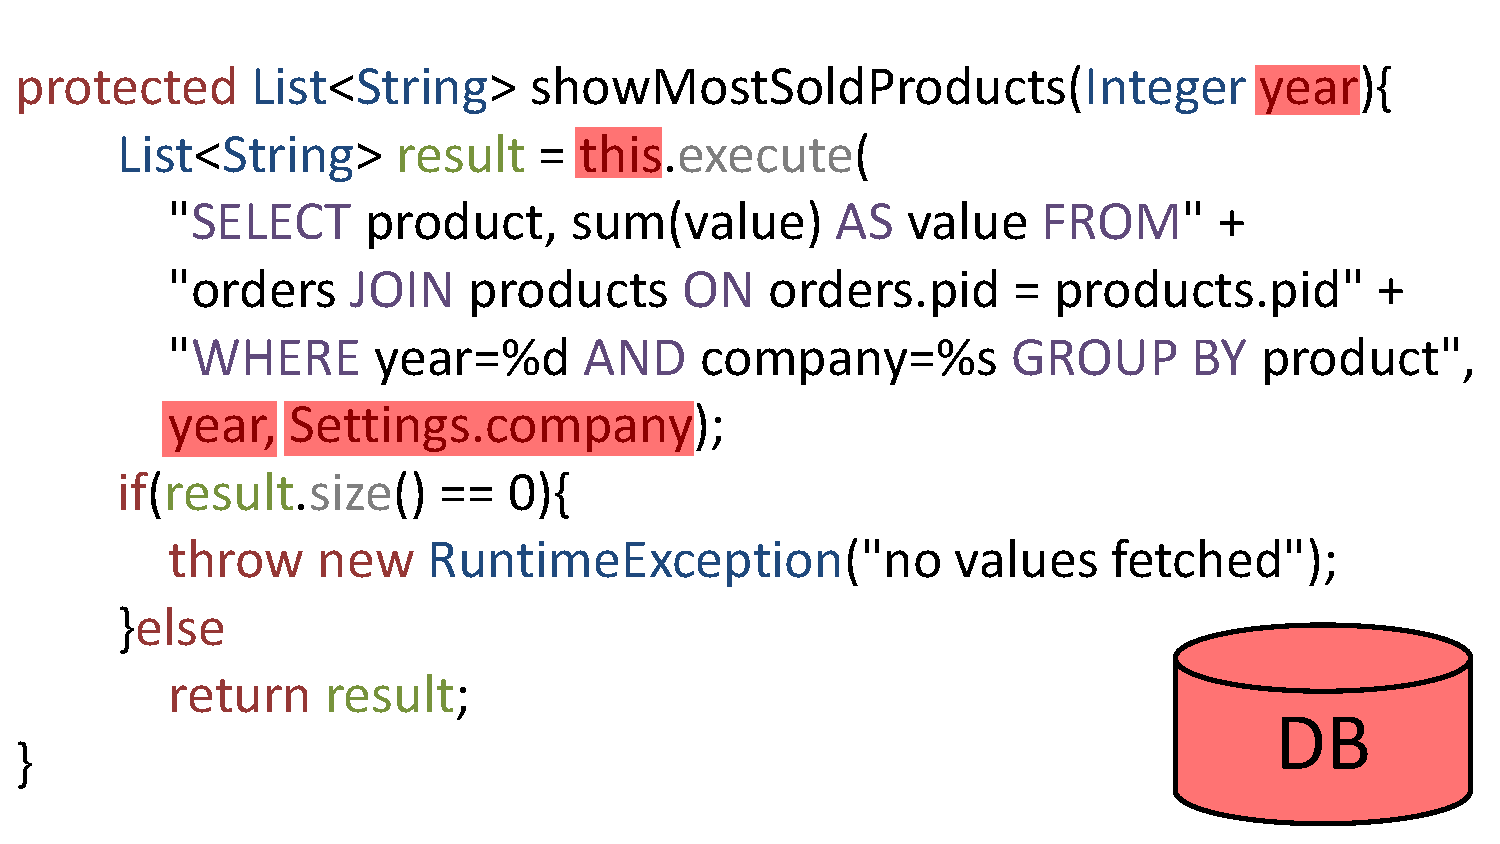
\includegraphics[width=\linewidth]{images/context}
    \caption{Running the statements of this Java method with its embedded SQL query requires all data highlighted in red: the parameter, accessible state, and the database.}
    \label{fig:context_recording}
\end{figure}

When a developer then interacts with a specific line in the method's body, we could use ordinary breakpoints to establish the necessary runtime data for that specific line of interest. 
Accessible state includes global state and, depending on the used programming language, also state from surrounding scopes as, for example, from surrounding functions or the receiver.
Snapshots of the database are necessary as methods that embedd queries might modify the database, potentially impeding subsequent runs of that method during the interactive development.

\subsection{Selecting Data Contexts}
The presented tracing approach generates potentially numerous data contexts for each method.
Given our tool traces live systems deployed at customers, each user interaction might lead to recorded data contexts for all method executions that such interactions trigger.
Further, even when our tool only traces tests once on replicated databases, particular methods might still be executed in multiple test cases or be called multiple times in single test cases as, for example, the case with methods called from loop bodies.
For these reasons, developers using our proposed environment might be confronted with many data contexts for each statement of interest.
Further, as data contexts from the same trace probably also overlap considerably, presenting all data contexts to the developer might reduce usability significantly.
Approaches addressing this issue include automatic selection of interesting samples after clustering all data contexts, preselection of interesting data contexts through expert users, and combinations of those two methods.
Clustering data contexts could be based on several dimensions, including:
\begin{itemize}
  \item size of the associated database snapshot
  \item control flow that lead to this context
  \item timestamp of this context
\end{itemize}
Nevertheless, even aiding through automatic clustering or manual preselections, our tools should probably also support developers in exploring the full extent of available contexts and make the final decision on which specific data context they want to use during development.

%Lauritz

%!TEX root = ../document.tex
\section{Open Questions} \label{sec:OPEN_QUESTIONS}
%Lauritz
In the future, we would like to investigate how seamless and helpful debugging of complete and partial SQL queries could be realized and integrated with our idea, whether and how actual hardware configurations could be considered as part of the data contexts from runtime, and how data contexts could be stored efficiently.

\subsection{Query Debugging}
Query debugging should be seamless.
It should provide immediate feedback while understanding and developing both application code and database queries.
Developers should, thus, not be required to use two tools to debug code.
They should not need to copy complete or parts of embedded queries from their application code to active database sessions.
Instead, an integrated debugger should be able to step through and evaluate both application code and embedded database queries without interrupting the developer through changing the user interactions or interface.
It should present return values, show basic profiling information, and allow to explore involved data.

Developers might also benefit from exploring the parts of queries.
However, as parts of SQL queries cannot necessarily be evaluated independently but might depent on other parts of the queries, developers potentially need to select multiple associated parts in conjunction.
For example, given the following query, the \texttt{WHERE} as well as the \texttt{SELECT} clause both rely on the \texttt{JOIN} in Line 2 of this example.
\lstset{language=SQL}
\begin{lstlisting}
  SELECT products.name, SUM (orders.price) as pricemake
  FROM orders JOIN products ON orders.pid=products.pid
  WHERE orders.year = 2012 and products.manufacturer = "HPI"
  GROUP BY product
\end{lstlisting}
An ideal data context debugger could aid developers also in selecting combinations of automatically identified meaningfull parts of database queries.

\subsection{Hardware Contexts}
Our idea focuses on showing actual results and basic profiling information right next to code and queries.
Assuming deadlock-free deterministic code, the results of queries should be independent of the underlying hardware.
However, the profiling information might depend significantly on the executing hardware.
Therefore, our approach would benefit from incorporating the impact of different hardware configurations.
Such hardware contexts should, thus, also be part of the data recorded at runtime.
We would focus further efforts in this directions on the capturing, storing, and application of hardware contexts.
Such hardware contexts could be used to either actually run statements on the associated hardware or to simulate the impact somehow.

A related question is whether data contexts should be tied to particular hardware contexts during our tracing.
Developers could gain insights from combining data contexts and hardware contexts freely to see how their application performs in many different situations.
However, bundling both contexts emphasizes optimizing performance for real usage.

\subsection{Context Representation}
As our approach potentially results in many similar data contexts for any given code section, storing data contexts could probably exploit these similarities between data contexts.
An implementation could identify similar data contexts, generate common base contexts, and, consequentely, store only the differences to those base contexts for each particular context.

As data contexts from the same traces potentially overlap with a high probability, marking data contexts with an identifier to indicate the used trace might allow to identify similar data contexts faster.

Further, the efficiency of storing data contexts could proably also leverage advanced database features as, for example, \emph{SAP HANA's Time Travel} feature~\footnote{\url{http://help.sap.com/hana/html/sql_create_table_history_time_travel.html}, retrieved March 12, 2013} that allows to reset the database to a specific moment in time.
Given this feature, an implementation would need to store only timestamps to establish the database part of data contexts instead of actual database snapshots.

%Lauritz

\section{Conclusion} \label{sec:CONCLUSION}
%HoD

\bibliography{references}
\bibstyle{splncs03}
\bibliographystyle{splncs03}

\end{document}
